\newcommand{\bankdistance}{4}
\tikzstyle{bank}=[
  draw,
  minimum width=1.5cm,
  minimum height=1cm,
  font=\huge
]
\tikzstyle{op}=[
  -latex,
  ultra thick
]

\newcommand{\drawbanks}[6]{{
  \newcommand{\banka}{#1}
  \newcommand{\bankb}{#2}
  \newcommand{\bankaa}{#3}
  \newcommand{\bankbb}{#4}
  \newcommand{\bankaaa}{#5}
  \newcommand{\bankbbb}{#6}

  \node[bank, label=above:{Replica $A$}] (a1) at (0,              0) {\banka};
  \node[bank                           ] (a2) at (0,             -3) {\bankaa};
  \node[bank                           ] (a3) at (0,             -6) {\bankaaa};
  \node[bank, label=above:{Replica $B$}] (b1) at (\bankdistance,  0) {\bankb};
  \node[bank                           ] (b2) at (\bankdistance, -3) {\bankbb};
  \node[bank                           ] (b3) at (\bankdistance, -6) {\bankbbb};

  \draw[op] (a1) -- (a2);
  \draw[op] (a2) -- (a3);
  \draw[op] (b1) -- (b2);
  \draw[op] (b2) -- (b3);
}}

\newcommand{\zigzag}[2]{{
  \newcommand{\banka}{#1}
  \newcommand{\bankb}{#2}

  \draw[red, op] ($(\banka) + (0, -0.7)$) -- ($(\bankb) + (0, -1.0)$);
  \draw[red, op] ($(\bankb) + (0, -1.0)$) -- ($(\banka) + (0, -1.3)$);
  \draw[red, op] ($(\banka) + (0, -1.3)$) -- ($(\bankb) + (0, -1.6)$);
  \draw[red, op] ($(\bankb) + (0, -1.6)$) -- ($(\banka) + (0, -1.9)$);
}}

\begin{frame}{Replicated Bank Account}
  \begin{center}
    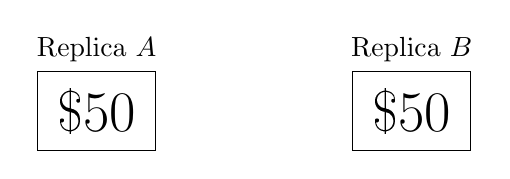
\begin{tikzpicture}
      \node[bank, label=above:{Replica $A$}] (a1) at (0, 0) {\$50};
      \node[bank, label=above:{Replica $B$}] (b1) at (\bankdistance, 0) {\$50};
    \end{tikzpicture}
  \end{center}
\end{frame}

\begin{frame}{Coordinating}
  \begin{center}
    \begin{tikzpicture}
      \drawbanks{\$50}{\$50}
                {\$60}{\$60}
                {\$80}{\$80}

      \draw[op] ($(a1) + (-2, 0)$) -- (a1) node[midway, above] {$+\$10$};
      \draw[op] ($(b1) + (+2, 0)$) -- (b1) node[midway, above] {$+\$20$};
      \draw[op] (a2) -- ($(a2) + (-2, 0)$) node[midway, above] {OK};
      \draw[op] (b3) -- ($(b3) + (+2, 0)$) node[midway, above] {OK};

      \zigzag{a1}{b1}
      \zigzag{a2}{b2}
    \end{tikzpicture}
  \end{center}
\end{frame}

\begin{frame}{Coordinating}
  \begin{center}
    \begin{tikzpicture}
      \drawbanks{\$50}{\$50}
                {\$20}{\$20}
                {\$20}{\$20}

      \draw[op] ($(a1) + (-2, 0)$) -- (a1) node[midway, above] {$-\$30$};
      \draw[op] ($(b1) + (+2, 0)$) -- (b1) node[midway, above] {$-\$40$};
      \draw[op] (a2) -- ($(a2) + (-2, 0)$) node[midway, above] {OK};
      \draw[op] (b3) -- ($(b3) + (+2, 0)$) node[midway, above] {NO};

      \zigzag{a1}{b1}
      \zigzag{a2}{b2}
    \end{tikzpicture}
  \end{center}
\end{frame}

\begin{frame}{Avoiding Coordination}
  \begin{center}
    \begin{tikzpicture}
      \drawbanks{\$50}{\$50}
                {\$60}{\$70}
                {\$80}{\$80}

      \draw[op] ($(a1) + (-2, 0)$) -- (a1) node[midway, above] {$+\$10$};
      \draw[op] ($(b1) + (+2, 0)$) -- (b1) node[midway, above] {$+\$20$};
      \draw[op] (a2) -- ($(a2) + (-2, 0)$) node[midway, above] {OK};
      \draw[op] (b2) -- ($(b2) + (+2, 0)$) node[midway, above] {OK};

      \draw[dashed, op] (a2) -- (b3) node[near start, sloped, above] {$+\$10$};
      \draw[dashed, op] (b2) -- (a3) node[near start, sloped, above] {$+\$20$};
    \end{tikzpicture}
  \end{center}
\end{frame}

\begin{frame}{Avoiding Coordination}
  \begin{center}
    \begin{tikzpicture}
      \drawbanks{\$50}{\$50}
                {\$20}{\$10}
                {-\$20}{-\$20}

      \draw[op] ($(a1) + (-2, 0)$) -- (a1) node[midway, above] {$-\$30$};
      \draw[op] ($(b1) + (+2, 0)$) -- (b1) node[midway, above] {$-\$40$};
      \draw[op] (a2) -- ($(a2) + (-2, 0)$) node[midway, above] {OK};
      \draw[op] (b2) -- ($(b2) + (+2, 0)$) node[midway, above] {OK};

      \draw[dashed, op] (a2) -- (b3) node[near start, sloped, above] {$-\$30$};
      \draw[dashed, op] (b2) -- (a3) node[near start, sloped, above] {$-\$40$};
    \end{tikzpicture}
  \end{center}
\end{frame}

\begin{frame}
  \begin{center}
    \Huge
    Deposits don't require coordination to maintain invariants, but withdrawals
    do.
  \end{center}
\end{frame}
